% Options for packages loaded elsewhere
\PassOptionsToPackage{unicode}{hyperref}
\PassOptionsToPackage{hyphens}{url}
%
\documentclass[
  a4paper,12pt]{extarticle}
\usepackage{lmodern}
\usepackage{amssymb,amsmath}
\usepackage{ifxetex,ifluatex}
\ifnum 0\ifxetex 1\fi\ifluatex 1\fi=0 % if pdftex
  \usepackage[T1]{fontenc}
  \usepackage[utf8]{inputenc}
  \usepackage{textcomp} % provide euro and other symbols
\else % if luatex or xetex
  \usepackage{unicode-math}
  \defaultfontfeatures{Scale=MatchLowercase}
  \defaultfontfeatures[\rmfamily]{Ligatures=TeX,Scale=1}
\fi
% Use upquote if available, for straight quotes in verbatim environments
\IfFileExists{upquote.sty}{\usepackage{upquote}}{}
\IfFileExists{microtype.sty}{% use microtype if available
  \usepackage[]{microtype}
  \UseMicrotypeSet[protrusion]{basicmath} % disable protrusion for tt fonts
}{}
\makeatletter
\@ifundefined{KOMAClassName}{% if non-KOMA class
  \IfFileExists{parskip.sty}{%
    \usepackage{parskip}
  }{% else
    \setlength{\parindent}{0pt}
    \setlength{\parskip}{6pt plus 2pt minus 1pt}}
}{% if KOMA class
  \KOMAoptions{parskip=half}}
\makeatother
\usepackage{xcolor}
\IfFileExists{xurl.sty}{\usepackage{xurl}}{} % add URL line breaks if available
\IfFileExists{bookmark.sty}{\usepackage{bookmark}}{\usepackage{hyperref}}
\hypersetup{
  hidelinks,
  pdfcreator={LaTeX via pandoc}}
\urlstyle{same} % disable monospaced font for URLs
\usepackage{longtable,booktabs}
% Correct order of tables after \paragraph or \subparagraph
\usepackage{etoolbox}
\makeatletter
\patchcmd\longtable{\par}{\if@noskipsec\mbox{}\fi\par}{}{}
\makeatother
% Allow footnotes in longtable head/foot
\IfFileExists{footnotehyper.sty}{\usepackage{footnotehyper}}{\usepackage{footnote}}
\makesavenoteenv{longtable}
\usepackage{graphicx}
\makeatletter
\def\maxwidth{\ifdim\Gin@nat@width>\linewidth\linewidth\else\Gin@nat@width\fi}
\def\maxheight{\ifdim\Gin@nat@height>\textheight\textheight\else\Gin@nat@height\fi}
\makeatother
% Scale images if necessary, so that they will not overflow the page
% margins by default, and it is still possible to overwrite the defaults
% using explicit options in \includegraphics[width, height, ...]{}
\setkeys{Gin}{width=\maxwidth,height=\maxheight,keepaspectratio}
% Set default figure placement to htbp
\makeatletter
\def\fps@figure{htbp}
\makeatother
\setlength{\emergencystretch}{3em} % prevent overfull lines
\providecommand{\tightlist}{%
  \setlength{\itemsep}{0pt}\setlength{\parskip}{0pt}}
\setcounter{secnumdepth}{-\maxdimen} % remove section numbering
\usepackage[spanish]{babel}
\usepackage{placeins}
\usepackage{graphicx} % Required to insert images
\usepackage{courier} % Required for the courier font
\usepackage{fixltx2e}
\usepackage{amsmath}
\usepackage{dsfont}
\usepackage{amssymb}
\usepackage{hyperref}
\usepackage{fancyhdr} % Required for custom headers
\usepackage{lastpage} % Required to determine the last page for the footer
\usepackage{extramarks} % Required for headers and footers
% Margins
\usepackage{geometry}
\geometry{
a4paper,
left=20mm,
right=20mm,
top=20mm,
bottom=20mm,
}

\linespread{1.1} % Line spacing

% Set up the header and footer
\pagestyle{fancy}
\lhead{} % Top left header
\chead{\hmwkClass\ (\hmwkClassTime): \hmwkTitle} % Top center head
\rhead{\hmwkInstitucional} % Top right header
\lfoot{\hmwkClassInstructor} % Bottom left footer
\cfoot{} % Bottom center footer
\rfoot{Página\ \thepage\ de\ \protect\pageref{LastPage}} % Bottom right footer
\renewcommand\headrulewidth{0.4pt} % Size of the header rule
\renewcommand\footrulewidth{0.4pt} % Size of the footer rule

\setlength\parindent{0pt} % Removes all indentation from paragraphs

% Encabezados y pies.

\newcommand{\hmwkTitle}{Clase 2 - Teoría} % Assignment title
\newcommand{\hmwkDueDate}{Abril 2020} % Due date
\newcommand{\hmwkClass}{Hidráulica Agrícola y Saneamiento} % Course/class
\newcommand{\hmwkClassTime}{1-2020} % Class/lecture time
\newcommand{\hmwkClassInstructor}{Mónica Fiore - Javier Clavijo} % Teacher/lecturer
\newcommand{\hmwkInstitucional}{FI-UBA} % Your name
\usepackage{lineno}
\linenumbers

\author{}
\date{}

\begin{document}

\hypertarget{hidraulica-agricola-y-saneamiento}{%
\section{HIDRAULICA AGRICOLA Y
SANEAMIENTO}\label{hidraulica-agricola-y-saneamiento}}

\hypertarget{facultad-de-ingenieruxeda-uba}{%
\subsubsection{Facultad de Ingeniería,
UBA}\label{facultad-de-ingenieruxeda-uba}}

\hypertarget{disponibilidad-de-agua}{%
\subsection{Disponibilidad de agua}\label{disponibilidad-de-agua}}

Uno de los factores determinantes de la salud humana es la
disponibilidad de agua dulce.

El crecimiento de la población, la industrialización y la expansión de
la agricultura de regadío en los últimos decenios han provocado un
aumento drástico en la demanda de agua.

\begin{figure}
\centering
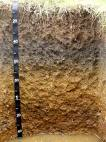
\includegraphics{./img/image1.jpeg}
\caption{Crecimiento poblacional por continente, \small Fuente:
\url{http://image.slidesharecdn.com/escenariosdedesarrollofuturo-140818163548-phpapp01/95/escenarios-de-desarrollo-futuro-52-638.jpg?cb=1408379816}}
\end{figure}

El consumo de agua con destino agrícola alcanza el 70\% de agua dulce.
En parte se debe a la aplicación de técnicas de riego inapropiadas.

\begin{figure}
\centering
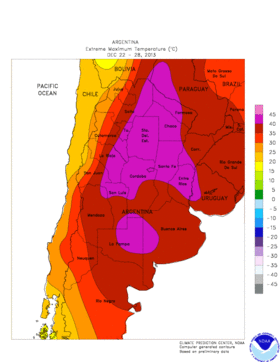
\includegraphics{./img/image4.png}
\caption{Uso del agua por continente y actividad, Fuente:
\url{http://www.fao.org/docrep/005/y3918s/y3918s03.htm}}
\end{figure}

\hypertarget{agua-para-la-agricultura}{%
\subsubsection{Agua para la
agricultura}\label{agua-para-la-agricultura}}

La agricultura, en especial la de riego, es el sector con mayor
extracción y uso~consuntivo de agua a nivel mundial.

\textbf{Usos consuntivos Son aquellos usos en los que el agua no puede
volver} \textbf{a utilizarse de la misma forma. Se la saca de su cauce
natural y no se} \textbf{la devuelve. Ejemplos: el agua que se utiliza
en agricultura,} \textbf{ganadería, industria.}

De acuerdo con estimaciones de la FAO (Food and Agriculture
Organization) en el 2011, el sector agrícola usó el 70\% de la
extracción total.

La aplicación del riego en una región depende de varios aspectos: La
disponibilidad de agua natural, en dónde el clima, el tipo del suelo y
el relieve juegan un papel preponderante . Las necesidades hídricas de
los diferentes cultivos, dependen directamente sus requerimiento
fisiológicos.

De acuerdo con estimaciones de la FAO en el 2011, de la superficie
cultivada, sólo el 19\% tenía infraestructura de riego, sin embargo
producía más del 40\% de los cultivos del mundo.

En los últimos 50 años, la población mundial se ha triplicado mientras
que el consumo de agua se ha sextuplicado. La demanda de agua para
consumo crece con el crecimiento de la población y con la mejora de sus
niveles de vida. Para satisfacer el aumento estimado de la demanda entre
2000 y 2030, se prevé que el cultivo de alimentos en los países en vías
de desarrollo aumente en 67\%.

\hypertarget{agua-para-la-industria}{%
\subsubsection{Agua para la industria}\label{agua-para-la-industria}}

A nivel mundial alrededor del 19\% del agua extraída se emplea en la
industria. De esta cantidad, más de la mitad se utiliza procesos de
enfriamiento de centrales termoeléctricas.

\hypertarget{agua-para-el-hogar}{%
\subsubsection{Agua para el hogar}\label{agua-para-el-hogar}}

\begin{longtable}[]{@{}ll@{}}
\toprule
Actividad & Consumo de agua\tabularnewline
\midrule
\endhead
Lavar la ropa & 60-100 litros\tabularnewline
Limpiar la casa & 15-40 litros\tabularnewline
Limpiar la vajilla a máquina & 18-50 litros\tabularnewline
Limpiar la vajilla a mano & 100 litros\tabularnewline
Cocinar & 6-8 litros\tabularnewline
Darse una ducha & 35-70 litros\tabularnewline
Bañarse & 200 litros\tabularnewline
Lavarse los dientes & 30 litros\tabularnewline
Lavarse los dientes (cerrando el grifo) & 1,5 litros\tabularnewline
Lavarse las manos & 1,5 litros\tabularnewline
Afeitarse & 40-75 litros\tabularnewline
Afeitarse (cerrando el grifo) & 3 litros\tabularnewline
Lavar el coche con manguera & 500 litros\tabularnewline
Descargar la cisterna & 10-15 litros\tabularnewline
Media descarga de cisterna & 6 litros\tabularnewline
Regar un jardín pequeño & 75 litros\tabularnewline
Riego de plantas domésticas & 15 litros\tabularnewline
Beber & 1,5 litros\tabularnewline
\bottomrule
\end{longtable}

Se estima que un habitante de un país desarrollado consume alrededor de
5 litros diarios en forma de alimentos y bebidas.

\hypertarget{agua-disponible}{%
\subsection{Agua disponible}\label{agua-disponible}}

En el mundo hay gran cantidad de agua dulce disponible, pero está
desigualmente repartida.

\begin{figure}
\centering
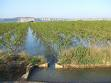
\includegraphics{./img/image9.jpeg}
\caption{Disponibilidad de agua dulce en paises representativos.}
\end{figure}

A esto deben añadirse las complejidades del manejo del agua que
atraviesa fronteras nacionales y los impactos cada vez mayores de las
sequías e inundaciones provocadas por el cambio climático.

\begin{figure}
\centering
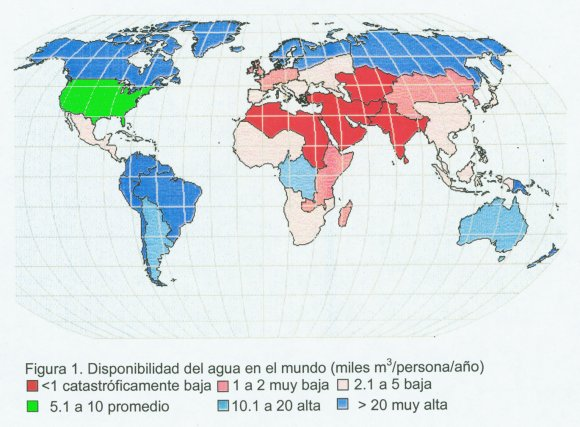
\includegraphics[width=6.25in,height=\textheight]{./img/image10.jpeg}
\caption{Disponibilidad de agua en el mundo categorizado, Fuente: World
Water Resources at the beginning of the 21st Century.}
\end{figure}

\hypertarget{se-suman-cambios-permanentes}{%
\subsubsection{Se suman cambios
permanentes}\label{se-suman-cambios-permanentes}}

En el Informe de Síntesis presentado en 2014 por el IPPC se destaca que:

\begin{enumerate}
\tightlist
\item
  La influencia humana en el sistema climático es clara, y las emisiones
  antropogénicas recientes de gases de efecto invernadero son las más
  altas de la historia. Los cambios climáticos recientes han tenido
  impactos generalizados en los sistemas humanos y naturales.
\item
  El calentamiento en el sistema climático es inequívoco, y desde la
  década de 1950 muchos de los cambios observados no han tenido
  precedentes en los últimos decenios a milenios. La atmósfera y el
  océano se han calentado, los volúmenes de nieve y hielo han disminuido
  y el nivel del mar se ha elevado.
\end{enumerate}

\begin{figure}
\centering
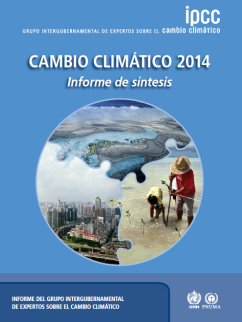
\includegraphics[width=2.60417in,height=\textheight]{./img/image11.png}
\caption{Informe del panel intergubernamental de Cambio Climático,
consultar en:
\url{https://archive.ipcc.ch/home_languages_main_spanish.shtml}}
\end{figure}

\begin{longtable}[]{@{}ll@{}}
\toprule
\endhead
Si explotamos el agua que se puede & Explotamos los\tabularnewline
renovar & recursos\tabularnewline
(en períodos de unos años) &\tabularnewline
Si utilizamos más agua que la que se puede & Explotamos las reservas
y\tabularnewline
renovar & producimos sobreexplotación\tabularnewline
\bottomrule
\end{longtable}

\hypertarget{agua-para-argentina}{%
\subsection{Agua para Argentina}\label{agua-para-argentina}}

Argentina presenta distribución desigual de sus recursos hídricos. 2/3
de su territorio esta constituido por regiones áridas y semiáridas y
sólo 1/3 es rico en fuentes de agua, principalmente superficiales, que
representan 84\% de las disponibilidades hídricas del país. Además de la
cantidad de agua, es relevante considerar la calidad del agua
disponible.

\begin{figure}
\centering
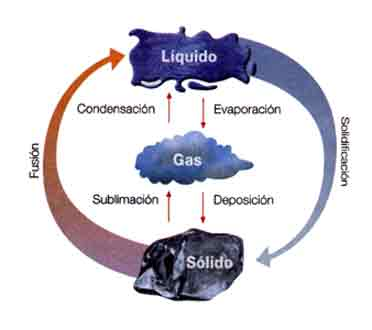
\includegraphics{./img/image12.jpeg}
\caption{Disponibilidad de agua en sistemas superficials, Fuente:
Instituto Nacional de Estadísticas y Censos (INDEC). Atlas digital de
los Recursos Hídricos Superficiales.
\url{http://www.ambiente.gov.ar/archivos/web/Indicadores/image/ids\%202010/sidsa\%202010/17-\%20disponibilidad\%20hidrica\%20por\%20cuenca\%20gr.jpg}}
\end{figure}

\begin{longtable}[]{@{}ll@{}}
\caption{Problemáticas derivadas de la distribución del agua dulce
Fuente: La cuestión del agua : consideraciones sobre el estado de
situación de los recursos hídricos de la Argentina . - 1a ed. - La Plata
: Universitaria de La Plata, 2011. 128 p.}\tabularnewline
\toprule
Región & Problemática\tabularnewline
\midrule
\endfirsthead
\toprule
Región & Problemática\tabularnewline
\midrule
\endhead
Árida y semiárida & Estrés hídrico por escasez y variabilidad estacional
de la oferta.\tabularnewline
& Limitación de posibilidades favorables para el\tabularnewline
& desarrollo de productos agrícolas de alto valor
relativo.\tabularnewline
& Conflictos por sobre-explotación de acuíferos\tabularnewline
& Pérdida de la capacidad productiva por salinización.\tabularnewline
Húmeda y subhúmeda & Degradación de la calidad de las aguas debido a la
contaminación\tabularnewline
& de aguas superficiales y subterráneas por vertido de efluentes no
tratados.\tabularnewline
& Presencia de altos contenidos de sales, exceso de arsénico y
flúor\tabularnewline
& (región norte y pampeana central).\tabularnewline
\bottomrule
\end{longtable}

\hypertarget{cambio-climuxe1tico}{%
\subsection{Cambio Climático}\label{cambio-climuxe1tico}}

Desde comienzos del siglo XX, el planeta ha evidenciado un aumento en la
temperatura media global, cuya tasa de calentamiento se ha intensificado
en las últimas décadas.

La influencia humana en el sistema climático juega un rol fundamental,
las recientes emisiones de origen antropogénico de gases de efecto
invernadero son las más altas de la historia (IPCC, 2014).

\begin{figure}
\centering
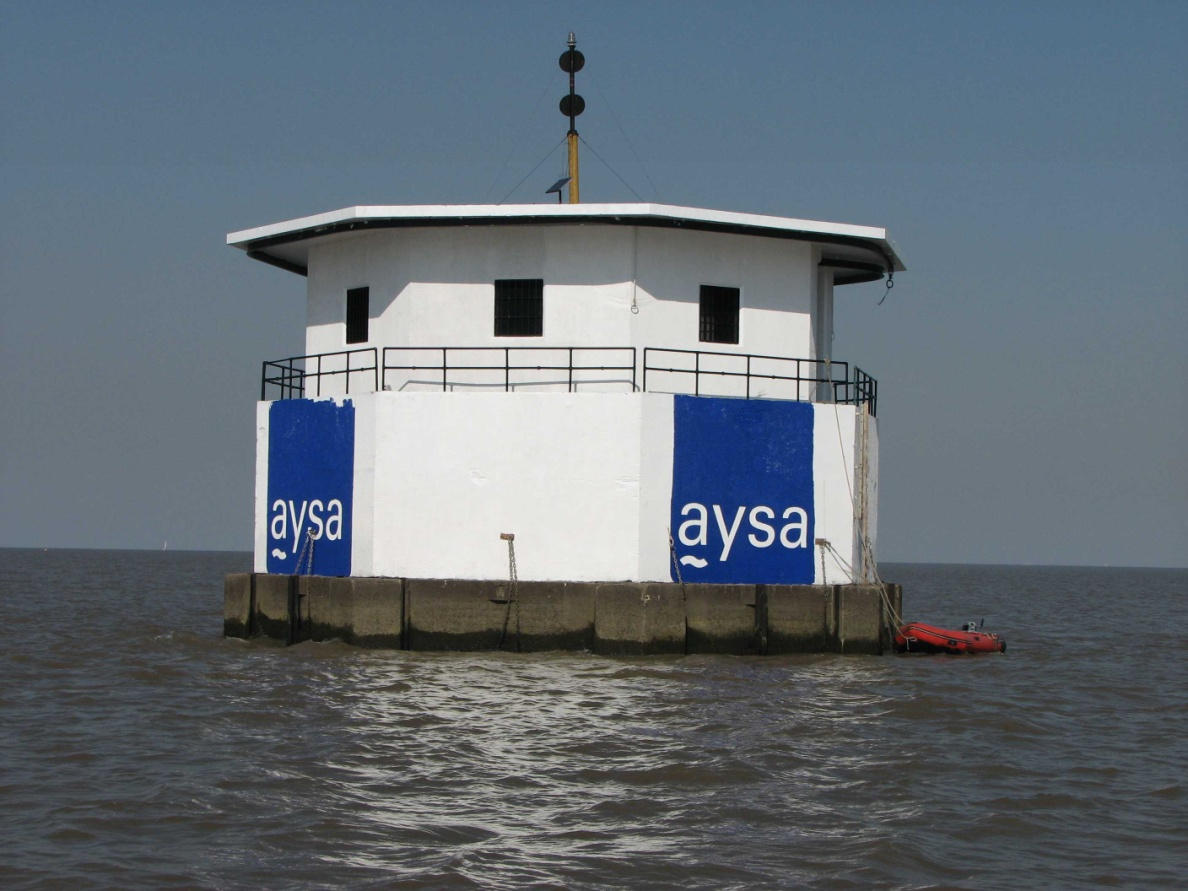
\includegraphics{./img/image13.jpeg}
\caption{Mapa de temperaturas de los últimos 50 años, en el que se
aprecian las diferencias entre ambos polos (Fuente: K. Armour)}
\end{figure}

\hypertarget{principales-gases-responsables-del-efecto.}{%
\subsubsection{Principales gases responsables del
efecto.}\label{principales-gases-responsables-del-efecto.}}

\begin{figure}
\centering
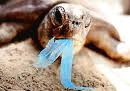
\includegraphics{./img/image14.jpeg}
\caption{Proporcion de los gases de efecto invernadero, Fuente:
\url{https://jpratt27.files.wordpress.com/2018/05/img_2518.jpg?w=620}}
\end{figure}

El \(CO_2\) por el momento es el principal~responsable del efecto
invernadero. Es el culpable de alrededor de las 3/4 partes del efecto de
calentamiento procedente de las actuales emisiones de gases de efecto
invernadero.

La concentración en la atmósfera es debido al uso de combustibles
fósiles como el carbón, el petróleo y el gas, aunque la deforestación es
también un contribuyente muy importante, dado que las hojas verdes
mediante la fotosíntesis son un regulador natural para este gas.

\begin{figure}
\begin{minipage}{0.48\textwidth}

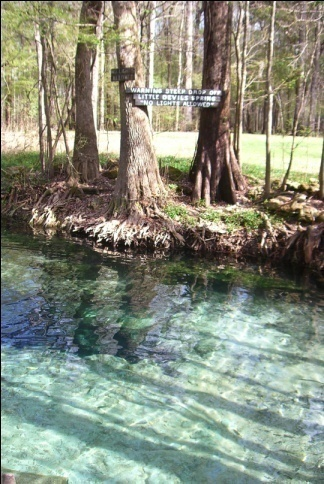
\includegraphics{./img/image16.jpeg}

\caption{ Temperatura vs. CO2, 1880-2013. (U.S. National Climate Assessment, via Climate Central) }
\end{minipage}%
\begin{minipage}{0.48\textwidth}

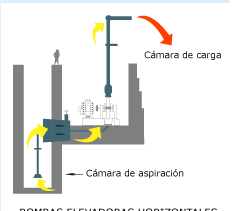
\includegraphics{./img/image18.png}

\caption{Evolución del $CO_2$ medido en la atmosfera, Fuente: http://cambioclimaticoglobal.com/wp-content/uploads/2013/08/co2-atmosferico-mauna-loa-abril-2013.png}
\end{minipage}
\end{figure}

El dióxido de carbono permanece en la atmósfera y los océanos durante
siglos. Esto significa que el mundo está comprometido con el cambio
climático continuo, independientemente de cualquier disminución temporal
de las emisiones.

El Metano, \(CH_4\), es un gas incoloro, inflamable y no tóxico. Su
origen se encuentra en las fermentaciones producidas por bacterias
anaerobias que se encuentran en zonas pantanosas, cultivos como el arroz
y en las emisiones del tracto intestinal del ganado.

Actualmente, el metano contribuye al Calentamiento Global con un 15\%.
Se sospecha que a fines del siglo XXI el efecto de este gas supere al
del \(CO_2\)

La ganadería vacuna y ovina repartidas por todo el planeta son las
responsables de casi una cuarta parte de todas las emisiones de metano
en el planeta.

\begin{figure}
\centering
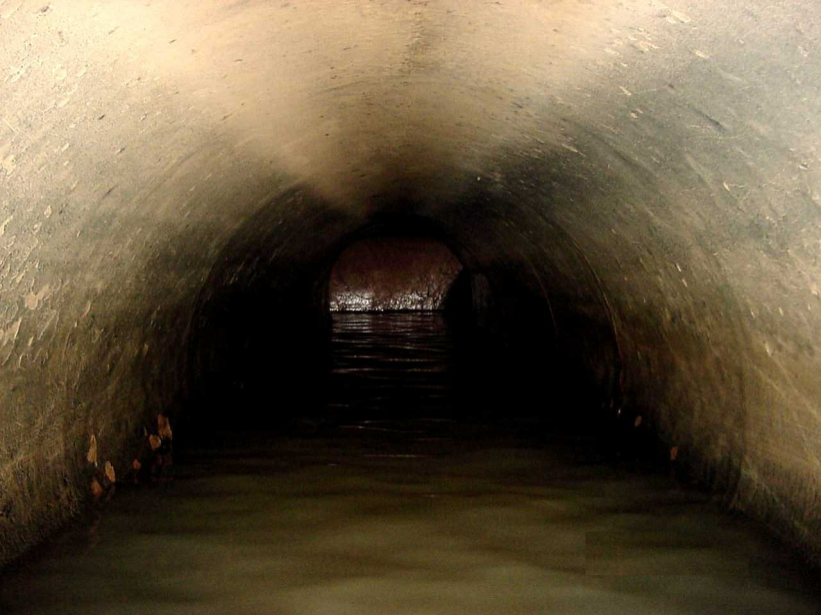
\includegraphics[width=6.25in,height=\textheight]{./img/image20.png}
\caption{Concentraciones de metano mensuales (circulos) desde 1983, con
la media movil en línea llena. Fuente: NOAA Climate.gov graph, based on
data from NOAA ESRL.}
\end{figure}

\begin{figure}
\centering

\includegraphics[width=6.25in,height=\textheight]{./img/image21.png}
\caption{Emisiones de carbono procidas por distinto tipo de ganadería}
\end{figure}

El \(N_2O\), Oxido nitroso, es un Gas invernadero que se produce
principalmente a través del uso masivo de fertilizantes nitrogenados en
la agricultura. También lo producen otras fuentes como las centrales
térmicas, tubos de escape de automóviles y motores de aviones, etc.

*Estudios realizados en 2018 en España por la Universidad Politéctinca
de Madrid indican que el uso de los fertilizantes con Zinc en cultivos
de secano reduce hasta en un 20\% las emisiones de oxido nitroso a la
atmósfera constituyendo una estrategia para mitigar la emisión de gases
de efecto invernadero.*

\begin{figure}
\centering
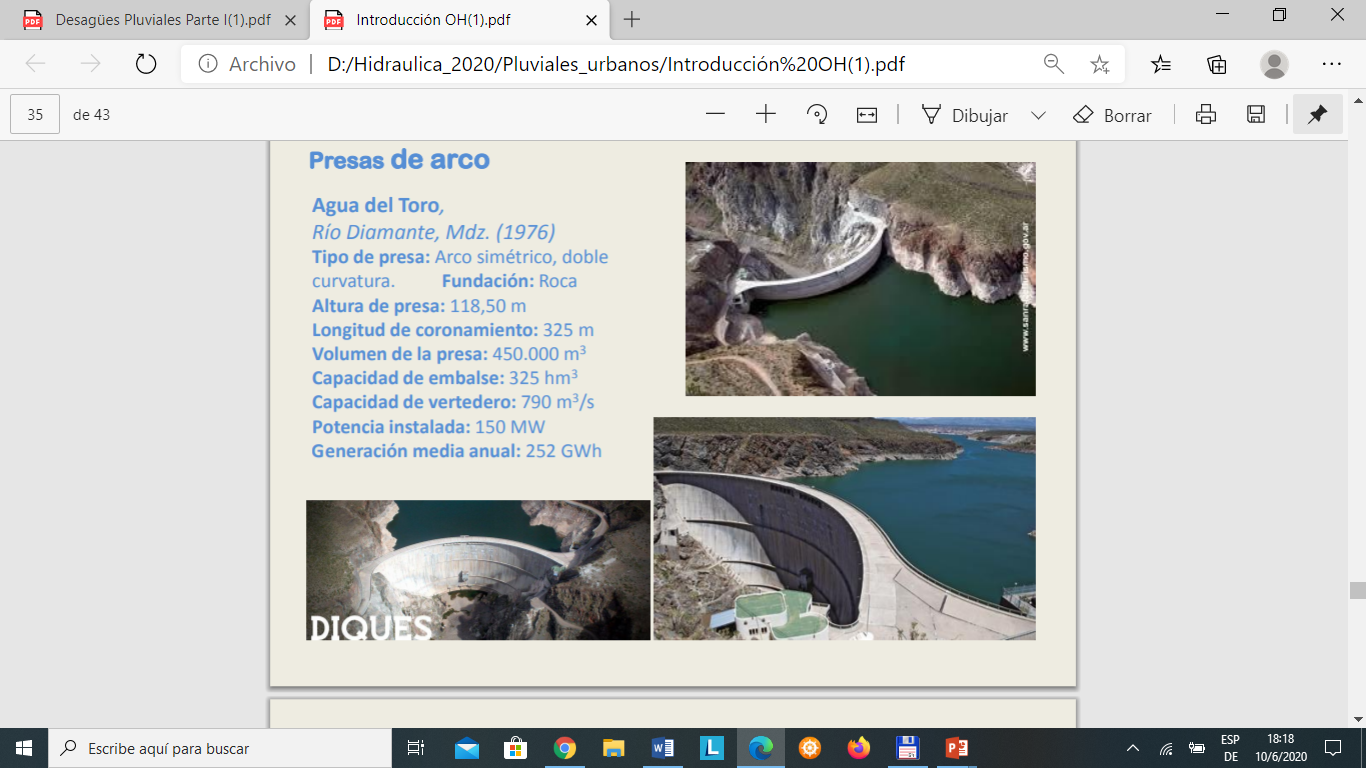
\includegraphics[width=4.6875in,height=\textheight]{./img/image23.png}
\caption{Tendencias en aumento de concentraciónes de los tres gases
mencionados: \(CO_2\), \(N_2O\) y \(CH_4\)}
\end{figure}

Cuando los agricultores añaden fertilizante nitrogenados al suelo para
estimular el crecimiento de las plantas, sólo la mitad de éste es
absorbido por la planta, el resto puede ser arrastrado por las aguas
subterráneas, o desviado como óxido nitroso u otros gases.

\begin{figure}
\centering
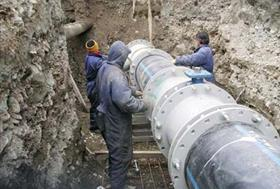
\includegraphics{./img/image24.jpeg}
\caption{Evolución del nitrógeno, desde el fertilizante hacia la
atmósfera. Fuente:
\url{https://jpratt27.files.wordpress.com/2018/05/img_2521.jpg?w=620}}
\end{figure}

Los clorofluorocarbonos (CFC) Son compuestos químicos artificiales que
se encuentran presentes en pequeñas concentraciones en la atmósfera pero
que son extremadamente potentes en su efecto invernadero. Tienen
múltiples usos industriales en sistemas de refrigeración, como
componentes de aerosoles, producción de aluminio y aislantes eléctricos
entre otros. Son los principales responsables del adelgazamiento de la
capa de ozono.

Los CFC fueron prohibidos hace 30 años por el Protocolo de Montreal por
sus efectos perjudiciales en la capa de ozono estratosférica.

\begin{figure}
\begin{minipage}{0.48\textwidth}

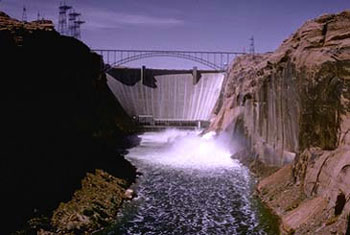
\includegraphics[width=3.125in,height=\textheight]{./img/image27.jpeg}

\caption{ Estructura de las moléculas de CFC}
\end{minipage}\hfill%
\begin{minipage}{0.48\textwidth}

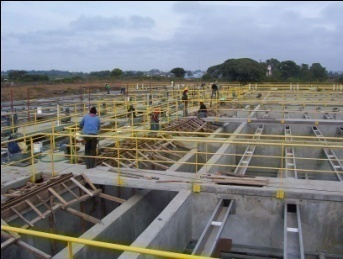
\includegraphics[width=3.125in,height=\textheight]{./img/image25.jpeg}

\caption{ Los CFCs han disminuido la concentración de ozono en la zona de la Antártida, que en el ultimo tiempo se ha estabilizado por primera vez, Fuente: https://www.meteorologiaenred.com/agujero-la-capa-ozono-se-estabiliza-primera-vez.html}
\end{minipage}
\end{figure}

\begin{figure}
\centering
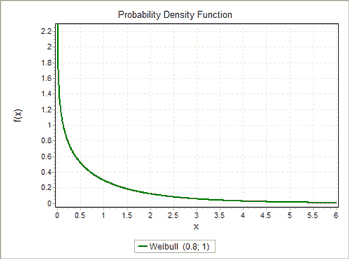
\includegraphics[width=4.16667in,height=\textheight]{./img/image26.png}
\caption{Evolución de los gases de efecto invernadero incluyendo CFC,
Fuente:
\url{https://upload.wikimedia.org/wikipedia/commons/thumb/6/6c/Chlorofluorocarbons_\%28space-filling_representation\%29.jpg/220px-Chlorofluorocarbons_\%28space-filling_representation\%29.jpg}}
\end{figure}

\hypertarget{efectos-en-la-temperatura}{%
\subsubsection{Efectos en la
temperatura}\label{efectos-en-la-temperatura}}

El calentamiento global ha originado cambios en el clima a nivel
regional y global.

\begin{itemize}
\tightlist
\item
  El incremento de temperatura
\item
  Mayor evaporación
\item
  Disminución de la humedad en superficie
\item
  Sequias mas largas e intensas
\end{itemize}

La temperatura de la tierra ha ido cambiando por causas naturales y
antropogénicas. Durante el siglo XX hubo 2 períodos de calentamiento,
uno entre 1910 -- 1945 y otro que se inicio en la década del 70 y
continua.

Las temperaturas globales de la superficie de la Tierra en el año 2019
fueron las segundas más cálidas desde que el registro comenzó en 1880.

A nivel mundial, las temperaturas de 2019 fueron superadas solo por las
de 2016 y continuaron la tendencia al calentamiento del planeta: los
últimos cinco años han sido los más cálidos de los últimos 140 años.

\begin{figure}
\centering
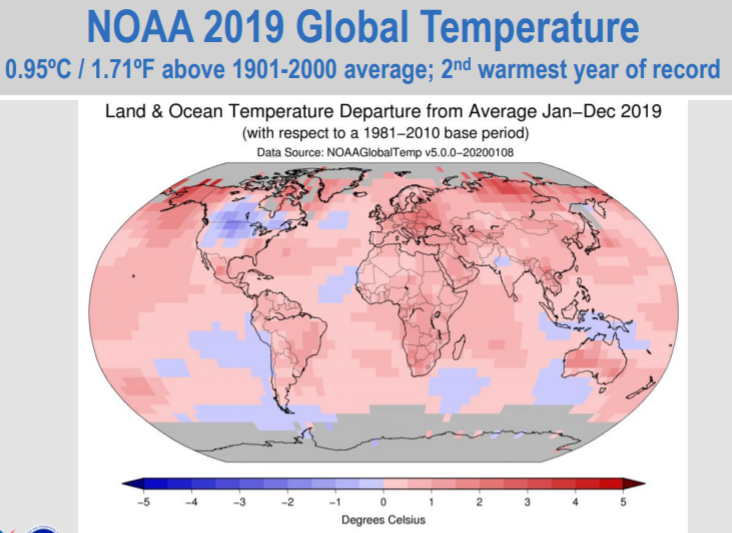
\includegraphics{./img/image28.png}
\caption{Temperatura Global 0.95ºC por encima del promedio 1901-2000.
Fuente:NOAA 2019
\url{https://ncdc.noaa.gov/sotc/briefings/20200115.pdf}}
\end{figure}

\begin{figure}
\centering
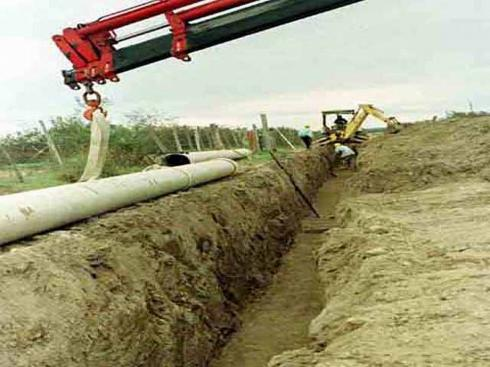
\includegraphics{./img/image29.jpeg}
\caption{Anomalías de temperatura anuales desde 1880 hasta 2019, con
respecto a la media de 1951-1980. Se ven pequeñas variaciones de un año
a otro, pero los cinco registros de temperatura muestran picos y valles
sincronizados entre sí. Todos indican un rápido calentamiento en las
últimas décadas, y todos señalan que la última década ha sido la más
cálida en el registro. Fuente: \url{https://data.giss.nasa.gov/gistemp}}
\end{figure}

El promedio de la temperatura global en el período 2001-2010 fue de
\(14,4^\circ\)

\begin{figure}
\centering
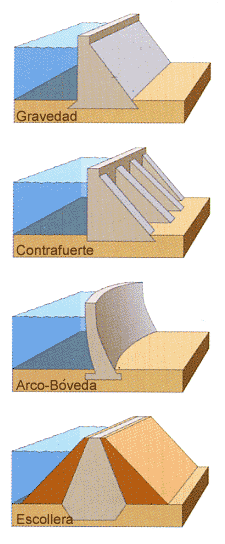
\includegraphics{./img/image30.png}
\caption{Temperatura por década obtenida combinando datos de temperatura
del aire a nivel mundial sobre la superficie terrestre y la superficie
del mar obtenidos a partir del promedio de 3 conjuntos de datos
independientes (HadCRU, NOAA y NASA-GISS). La línea gris horizontal
indica el valor medio a largo plazo para el período 1961-1990 (14 °C).
Fuente:
\url{http://4.bp.blogspot.com/-dcKGnsh-JfA/UdWpxu7qPKI/AAAAAAAAFJs/YWphQy2LAOQ/s1600/temperatures+per+decennis.gif}}
\end{figure}

La temperatura media de la superficie de la Tierra durante el siglo XX,
medida con termómetros en superficie, subió aproximadamente unos 0.6 ºC.

Este ascenso no fue uniforme, ni en forma temporal ni espacial. El
aumento se produjo en dos períodos, 1910-1945 y 1978-1998. Entre estos
dos períodos 1945-1978, la temperatura media global de la superficie
terrestre tendió a estabilizarse e incluso a tener una tendencia
negativa.

Esta evolución desigual probablemente indique que han existido factores
naturales, y no sólo antrópicos, en las variaciones térmicas,
especialmente durante el primer período de ascenso (1910-1945), ya que
en ese lapso las emisiones de CO2 y de otros gases invernadero eran
todavía muy escasas.

Las diferencias regionales en la evolución térmica son importantes. No
hay que olvidar que la temperatura media global es una media que suele
contabilizar fenómenos simultáneos de calentamiento en unas zonas y de
enfriamiento en otras.

\hypertarget{temperaturas-diurnas-y-nocturnas}{%
\subsubsection{Temperaturas diurnas y
nocturnas}\label{temperaturas-diurnas-y-nocturnas}}

Otra de las características importantes de estos cambios es que,
especialmente en el hemisferio Norte, las temperaturas mínimas nocturnas
han experimentado un ascenso de 0.8ºC, que es mucho mayor que el de las
temperaturas máximas diurnas, que es de 0.2ºC.

En el futuro, un calentamiento global que estuviese causado por el
incremento de las temperaturas mínimas nocturnas (sobre todo,
invernales) podría ser considerado de consecuencias benignas para la
humanidad, e incluso beneficiosas.

Se ha comprobado estadísticamente que a lo largo del siglo XX en casi
todo el mundo han disminuido los días de helada y se considera como muy
probable que las olas de frío hayan también disminuido (Lockwood, 1998;
Easterling, 2000).

\hypertarget{la-temperatura-media-global}{%
\subsubsection{La temperatura media
global}\label{la-temperatura-media-global}}

Durante el siglo pasado la temperatura media mundial se incrementó casi
0.7 °C, y la magnitud de este aumento no tiene precedentes por lo menos
durante el ultimo milenio. La distribución espacial de estos cambios no
fue homogénea, sino que los mayores aumentos ocurrieron sobre los
continentes, especialmente en latitudes altas del HN.

La inhomogeneidad en los cambios de temperatura altero los gradientes
térmicos.

Alteración en la circulación general de la atmosfera y por lo tanto en
los patrones de distribución de las precipitaciones.

\hypertarget{efecto-en-las-precipitaciones.}{%
\subsubsection{Efecto en las
precipitaciones.}\label{efecto-en-las-precipitaciones.}}

\begin{figure}
\centering
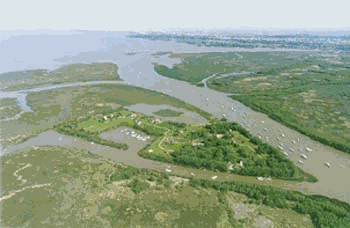
\includegraphics{./img/image31.png}
\caption{Tendencias porcentuales de las precitaciones anuales durante el
siglo XX. Gris claro corresponden a disminuciones y gris oscuro a
aumentos. El área de los círculos se relaciona con la magnitud de la
tendencia. (Fuente: IPCC, 2003).}
\end{figure}

Se observa una preponderancia de los aumentos de precipitación sobre los
continentes, principalmente en latitudes medias y altas. Sin embargo,
hay tendencias decrecientes en muchas zonas desérticas, incrementando
aún más el contraste regional. Por ejemplo al sur de Sudamérica, donde
la cordillera de los Andes divide dos regiones fuertemente
contrastantes, se observa un aumento de un 25\% en las precipitaciones
al este y una disminución del 50\% al oeste (Serio, 2006).

\begin{figure}
\centering
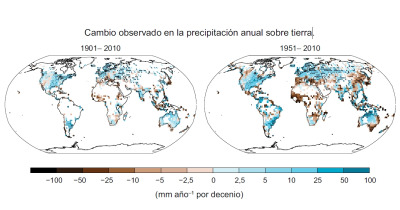
\includegraphics{./img/image32.jpeg}
\caption{Cambios observados en la precipitación, entre 1901 y 2010, y
entre 1951 y 2010 (IPCC, 2014). Fuente:
\url{http://40.media.tumblr.com/7159552d47859adcd31aeb36e8d065a6/tumblr_npssm2Ed8G1qb9oj8o1_400.jpg}}
\end{figure}

\begin{figure}
\begin{minipage}{0.48\textwidth}

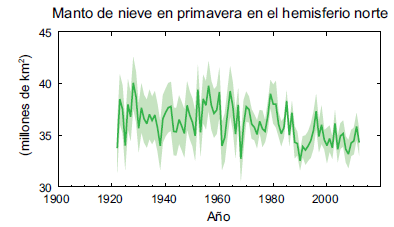
\includegraphics{./img/image33a.png}

\end{minipage}\hfill%
\begin{minipage}{0.48\textwidth}

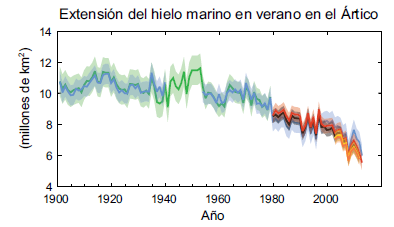
\includegraphics{./img/image33b.png}

\end{minipage}
\begin{minipage}{0.48\textwidth}

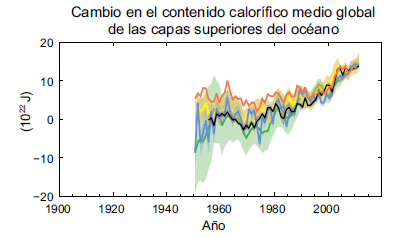
\includegraphics{./img/image33c.png}

\end{minipage}\hfill%
\begin{minipage}{0.48\textwidth}

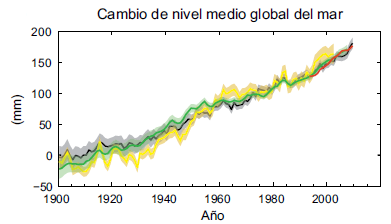
\includegraphics{./img/image33d.png}

\end{minipage}
\caption{ Otros indicadores del cambio climático }
\end{figure}

\hypertarget{cambios-en-las-precipitaciones}{%
\subsubsection{Cambios en las
precipitaciones}\label{cambios-en-las-precipitaciones}}

Por cada grado centígrado que sube la temperatura, la capacidad de
contener vapor de agua en la atmosfera se incrementa en un 7\%. Esto
produce mayor contenido de agua en la atmósfera. Hace que las tormentas
sean mas intensas. Aun cuando la precipitación total está disminuyendo.

\hypertarget{cambios-relevantes-para-la-regiuxf3n.}{%
\subsubsection{Cambios Relevantes para la
Región.}\label{cambios-relevantes-para-la-regiuxf3n.}}

Del análisis de datos de prec. y temp. máximas y mínimas surge que el SE
de América de Sur es una de las regiones del mundo en donde la tendencia
de lluvia caída en la ultima centuria es mayor.

En Argentina en los últimos 40 años la precipitación anual se incremento
entre un 10\% y un 40\%, según la región.

También han ocurrido algunas fluctuaciones del clima cuya relación con
el cambio climático global no siempre es directa. La temperatura media
anual aumentó en casi todo el país, aunque no de manera homogénea. El
aumento fue de 0,2 °C en promedio en el Norte y de alrededor de 1 °C en
la Patagonia (Hoffmann et al., 1997).

En general, las precipitaciones aumentaron en la franja central y este
(Castañeda y Barros, 1994) y disminuyeron sobre y al oeste de la
cordillera.

Los cambios en la precipitación y la temperatura son mas evidentes
durante los meses de verano y primavera. Durante el verano y la
primavera la precipitación aumentó, la temperatura máxima disminuyo y la
mínima aumento.

Dada la extensión de la Argentina y la variedad de su clima, el cambio
climático incidirá en forma diferente en las distintas regiones del país
.

La región andina subtropical es la que mayores cambios de temperatura ha
registrado desde 1960 y sobre la que se proyecta el mayor calentamiento
durante el resto del siglo, lo que conducirá a un escenario de creciente
estrés hídrico, y la probable extinción local de algunas de las especies
menos tolerantes a estas nuevas condiciones.

En la región pampeana, que es la de mayor importancia en la agricultura
nacional, los modelos de productividad indican que en el futuro cercano
y considerando el efecto del \(CO_2\), los rendimientos medios de soja y
maíz aumentarían en forma considerable y moderada respectivamente,
mientras que el cultivo de trigo sufriría leves reducciones con
diferencias geográficas; las pérdidas de productividad de este cereal
serán importantes en Córdoba y Santa Fe, mientras que el Sur y Oeste de
la provincia de Buenos Aires y la zona productiva de La Pampa se verían
beneficiados.

Los humedales alto andino y de la Puna tenderían a la reducción de sus
áreas totales, afectando a los animales que dependen de estos hábitats,
como las aves acuáticas y los grandes herbívoros.

En la Patagonia, la tendencia hacia mayores temperaturas y
precipitaciones menores, aun en el caso de reducciones pequeñas,
configura una tendencia hacia mayor aridez.

La tendencia a la recesión de los glaciares continuaría durante este
siglo, de acuerdo con las proyecciones de aumento de temperatura en
todos los escenarios de concentración de GEI.

\begin{figure}
\centering
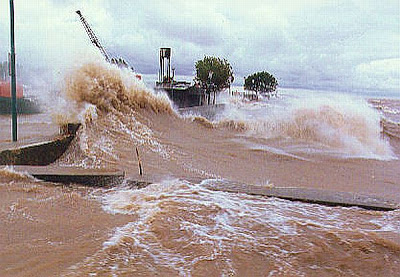
\includegraphics{./img/image36.jpeg}
\caption{Diferencias evidentes en el manto de nieve en la patagonia.}
\end{figure}

Los modelos de producción ganadera proyectan para fin de siglo
reducciones de la producción de carne bovina en el Norte de la región
Pampeana, estabilidad en el centro de la región y aumentos en la zona
oeste.

Estos cambios se producirían principalmente por el efecto de los cambios
del clima en la producción de forraje. Otro cambio importante sería el
desplazamiento geográfico de las zonas ganaderas.

\begin{figure}
\centering
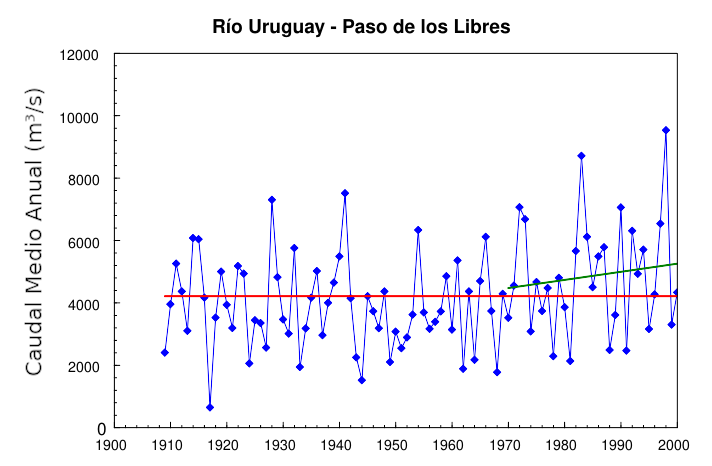
\includegraphics[width=2.08333in,height=\textheight]{./img/image37.png}
\caption{Existen numerosos Estudios sobre el efecto y la mitigación del
cambio climático en la agricultura, Fuentes:
\url{https://ced.agro.uba.ar/ubatic/?q=node/79}}
\end{figure}

La región ganadera de clima templado, ubicada al sur de la isoterma de
26°C durante el mes más cálido, se reduciría paulatinamente, a medida
que avanzan las condiciones más cálidas, ocupando a fines del siglo,
solo el centro- sur y centro-oeste de la provincia de Buenos Aires y el
centro de La Pampa.

La región de ganadería tropical, ubicada al N de la isoterma de 26°C
durante el mes más cálido, se desplazaría paulatinamente hacia el E en
su límite N y hacia el SO en su zona S y media.

\begin{figure}
\centering
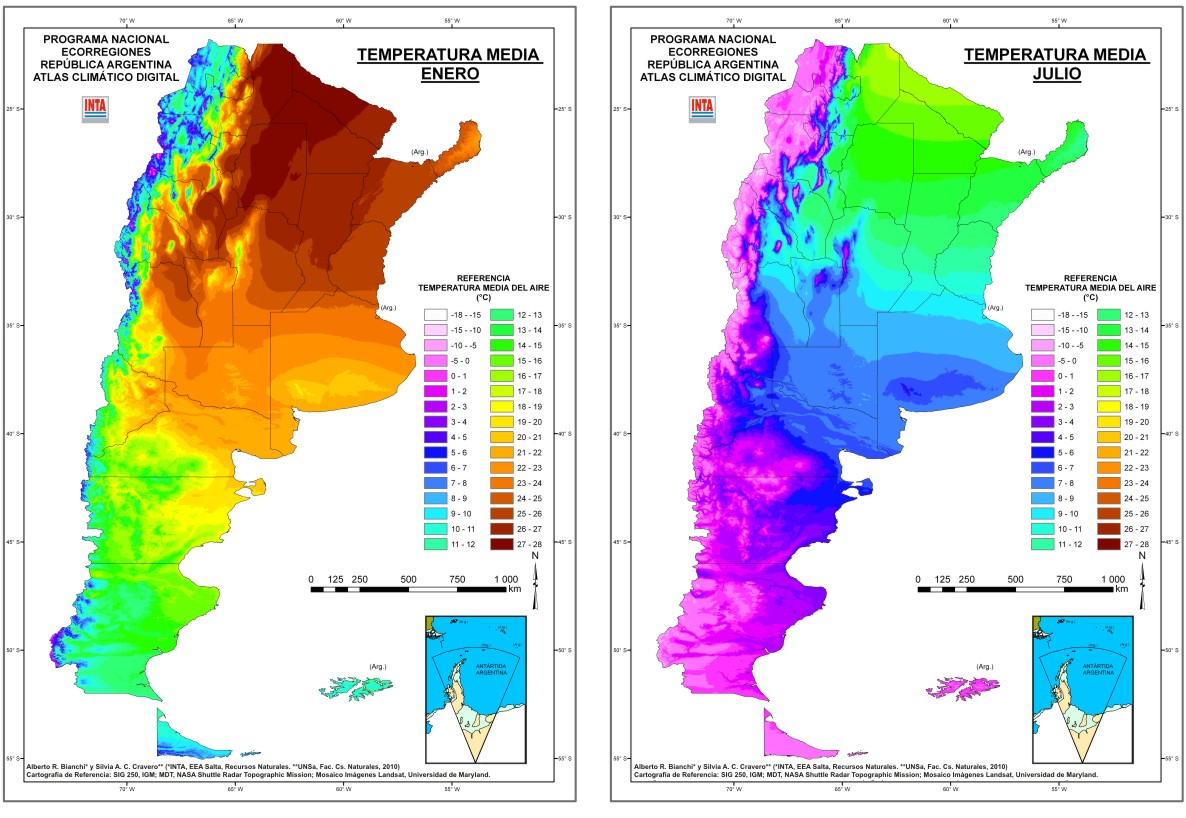
\includegraphics{./img/image38.png}
\caption{Temperaturas medias de referencia en la argentina. Fuente: INTA
\url{https://inta.gob.ar/documentos/atlas-climatico-digital-de-la-republica-argentina}}
\end{figure}

\hypertarget{nivel-del-mar}{%
\subsection{Nivel del mar}\label{nivel-del-mar}}

Uno de los impactos más importante del cambio climático en este siglo es
la elevación del nivel del mar. Tanto a nivel global como regional se ha
detectado un incremento relativo que varía según la zona analizada.

\begin{figure}
\centering
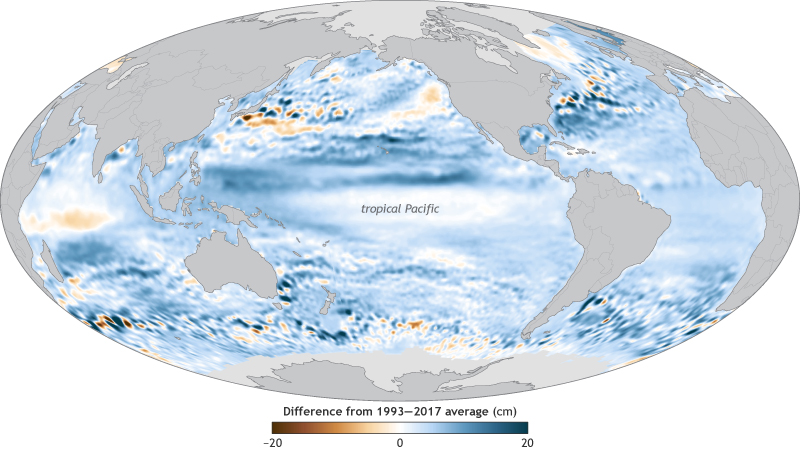
\includegraphics{./img/image39.jpeg}
\caption{Mapa de nivel medio del mar para 2017 respecto del promedio
1993-2017. Fuente:NOAA Climate.gov map, adapted from Figure 3.16a in
''State of the Climate in 2017''}
\end{figure}

\null\hfill\begin{minipage}{0.8\textwidth}

El nivel medio del mar se puede calcular a partir de registros de
estaciones mareográficas, realizando la media aritmética de niveles
horarios de marea (o alturas equiespaciadas con un intervalo menor)
durante un período de tiempo adecuado, lo suficientemente largo para
eliminar la influencia de la marea.

La evolución del nivel medio ha sido estudiada en las últimas dos
décadas del siglo XX a escala global y regional no siendo todas las
regiones afectadas de la misma forma.

Los modelos climáticos, los datos satelitales y las observaciones
mareográficas muestran que el nivel del mar no sube uniformemente en
todo el mundo, siendo en algunas regiones, las tasas muy superiores al
promedio mundial, mientras que en otras regiones el nivel del mar
disminuye (IPCC, 2014).

\emph{IPCC, 2014: Cambio climático 2014: Informe de síntesis.}

\emph{Contribución de los Grupos de trabajo I, II y III al Quinto
Informe de} \emph{Evaluación del GrupoIntergubernamental de Expertos
sobre el Cambio} \emph{Climático {[}Equipo principal de redacción, R.K.
Pachauri y L.A. Meyer} \emph{(eds.){]}. IPCC, Ginebra,Suiza, 157 págs.}

\end{minipage}

El quinto reporte del IPCC (AR5) determino que más del 90\% de la
energía térmica extra en el sistema climático es absorbida y retenida en
el océano. Como resultado, el océano global se calienta y se vuelve más
ácido (debido a la retención de CO\textsubscript{2} y al aumento de
temperatura del océano). Otra cosa para destacar es que existen
evidencias de que el océano está perdiendo oxígeno (Oschlies et al.,
2018).

El nivel del mar ha ido subiendo en el último siglo, y la tasa ha
aumentado en las últimas décadas. Desde 1993, las mediciones altimetría
permitieron analizar la evolución del nivel del mar a escala espacial y
temporal.

\begin{longtable}[]{@{}ll@{}}
\toprule
Período & Tendencia\tabularnewline
\midrule
\endhead
1901 - 1990 & 2,1 mm/año\tabularnewline
1970 - 2015 & 3,2 mm/año\tabularnewline
2005 - 2015 & 3,6 mm/año\tabularnewline
\bottomrule
\end{longtable}

En el período 1901 - 2010, el nivel medio del mar a escala global
aumentó 0,19 {[}0,17 a 0,21{]} m.

Existen dos mecanismos principales que contribuyen al ascenso del nivel
del mar.

\begin{itemize}
\tightlist
\item
  la dilatación térmica: el agua del océano se expande al calentarse.
\item
  la fusión de los grandes depósitos de hielo terrestre, como los
  casquetes de hielo y glaciares.
\end{itemize}

Tanto a nivel global como regional, se ha detectado un incremento del NM
que varía según la zona analizada. Cada región del planeta presenta
tendencias originadas por efectos climáticos, oceánicos y geológicos.

El nivel relativo del mar se define como el nivel del mar que se observa
con respecto a un marco de referencia ubicado en tierra.

Si se considera el período correspondiente a las mediciones altimétrica
registradas durante 1993-2016, el nivel medio del mar a escala global ha
aumentado a un ritmo de 3,3 mm/año.

Para comprender la configuración actual de las costas y la plataforma
continental debemos conocer las causas que originan las variaciones.

Básicamente las variaciones relativas del nivel del mar del orden de
decenas de metros se deben a:

\begin{itemize}
\tightlist
\item
  Variaciones en el volumen del agua
\item
  Variaciones verticales de las placas
\end{itemize}

\begin{figure}
\centering
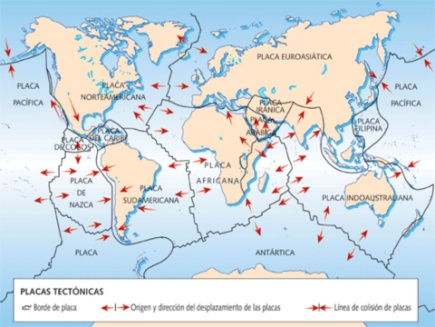
\includegraphics[width=4.16667in,height=\textheight]{./img/image42.jpeg}
\caption{El movimiento de las placas tectónicas también se da en la
componente altura, en el proceso conocido como Isostasia.}
\end{figure}

\hypertarget{variaciones-del-nmm-asociadas-a-las-glaciaciones}{%
\subsubsection{Variaciones del NMM asociadas a las
glaciaciones}\label{variaciones-del-nmm-asociadas-a-las-glaciaciones}}

Durante el último medio millón de años el NMM del mar experimentó
ascensos y descensos debido al retroceso o avance de los glaciares.

Una Glaciación es un periodo de larga duración en el que las
temperaturas globales de la tierra descienden de forma generalizada,
como resultado de este proceso el hielo de los casquetes polares se
extiende hasta cubrir grandes áreas continentales.

\begin{figure}
\centering
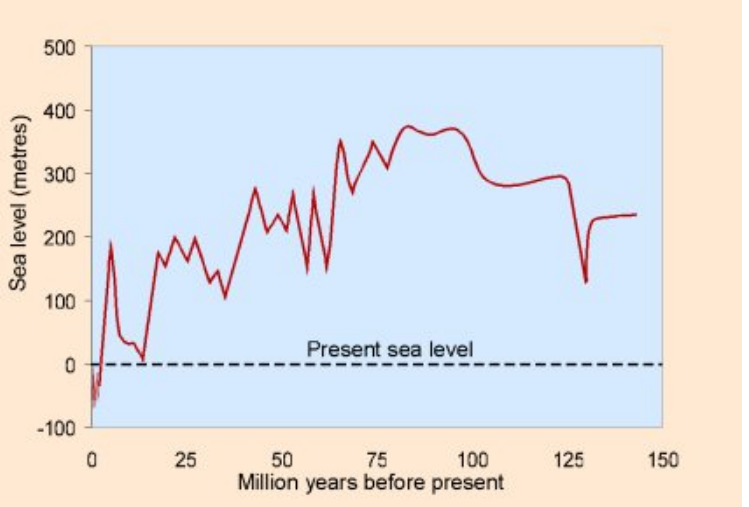
\includegraphics[width=3.64583in,height=\textheight]{./img/image44.png}
\caption{Estimacion de Niveles del mar global durente los últimos 150
milones de años}
\end{figure}

El Glaciar Viedma es un ejemplo representativo de lo que está sucediendo
en todos los glaciares del Sur. Según estimaciones hechas el Glaciar
Viedma perdió aproximadamente 50 m en altura y retrocedió 1 km en los
últimos 70 años.

Las proyecciones de la temperatura para este siglo hacen prever que la
actual tendencia recesiva de los glaciares de la región continuará, en
forma acelerada, acompañando las tendencias térmicas.

Casi todos los glaciares de los Andes Patagónicos han estado
retrocediendo durante las últimas décadas debido al aumento de la
temperatura y en algunas zonas por la menor precipitación.

El Glaciar Upsala retrocedió 13,4 km en un acelerado proceso de pérdida
de hielo ocurrido entre los años 1997 y 2003.

El Glaciar Upsala tiene una sup. aproximada de 870 km², una longitud de
60 km y un ancho promedio de 10 km. El frente del Glaciar Upsala, al
igual que el frente del Perito Moreno, desemboca en el Lago Argentino.

\begin{figure}
\centering
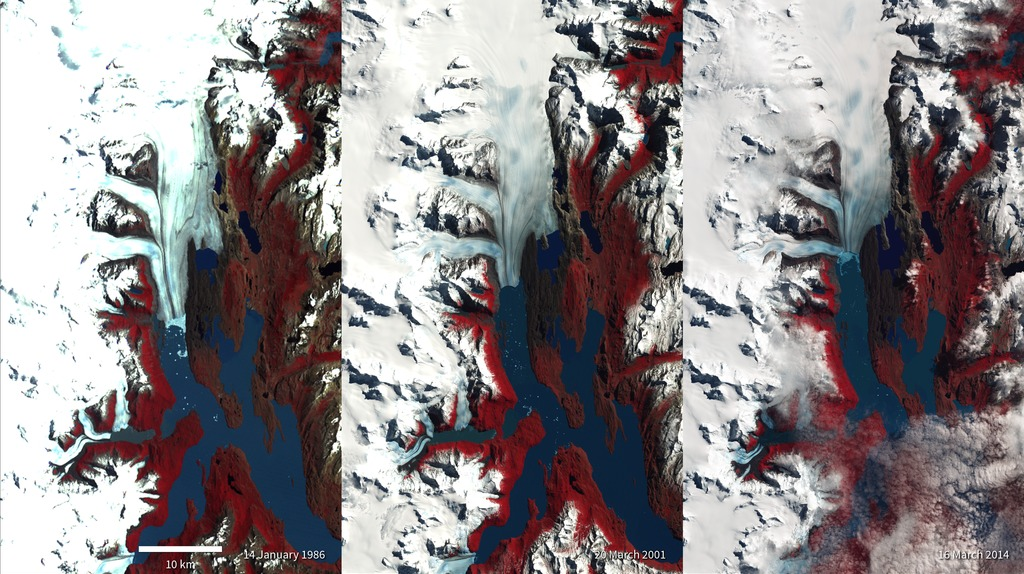
\includegraphics[width=6.25in,height=\textheight]{./img/image46.jpg}
\caption{Glacial Upsala, Comparativa 1986-2001-2014. Fuente NASA:
\url{https://svs.gsfc.nasa.gov/30549}}
\end{figure}

Las áreas costeras caracterizadas por poseer una rica diversidad de
ecosistemas y por tener grandes concentraciones de población serán las
más vulnerables al ascenso del nivel del mar, siendo las más bajas las
más desprotegidas.

¿Por qué es importante estudiar el Nivel Medio del Mar? La población
mundial se distribuye de manera desigual

\begin{figure}
\centering
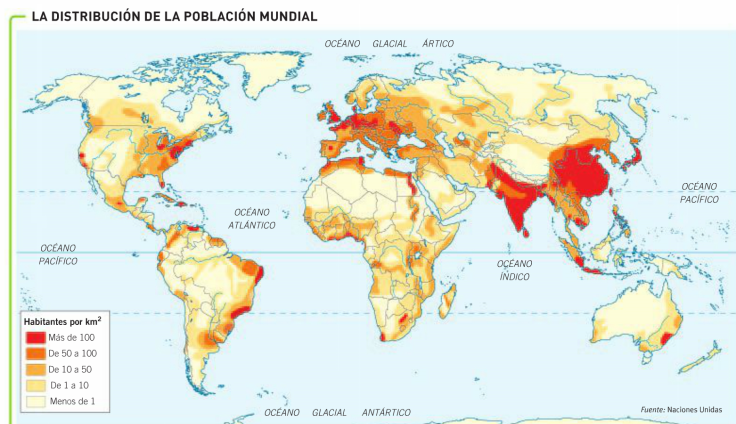
\includegraphics{./img/image47.png}
\caption{Distribución de la población a nivel global, nótese la
concentación en áreas costeras.}
\end{figure}

Los cambios del nivel del mar tienen aparejados impactos en las ciudades
balnearias tanto en bienes privados (viviendas) o públicos
(infraestructura), como, por ejemplo, eventuales aumentos de la altura
de las olas (Dragani y coautores, 2010).

\begin{figure}
\centering
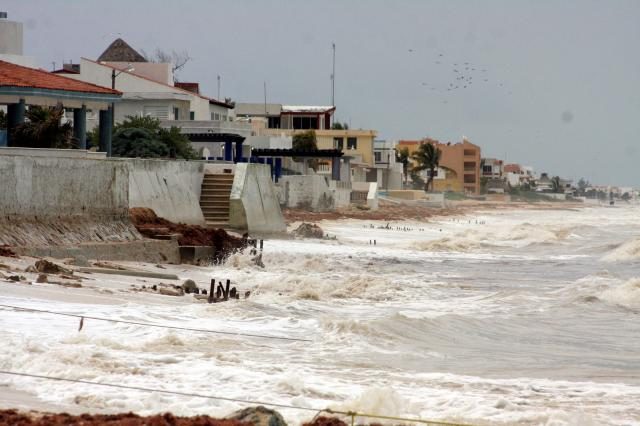
\includegraphics[width=3.64583in,height=\textheight]{./img/image48.jpeg}
\caption{Erosión Costera en Mar del Tuyú, Pcia. de Bs. As.}
\end{figure}

\begin{figure}
\centering
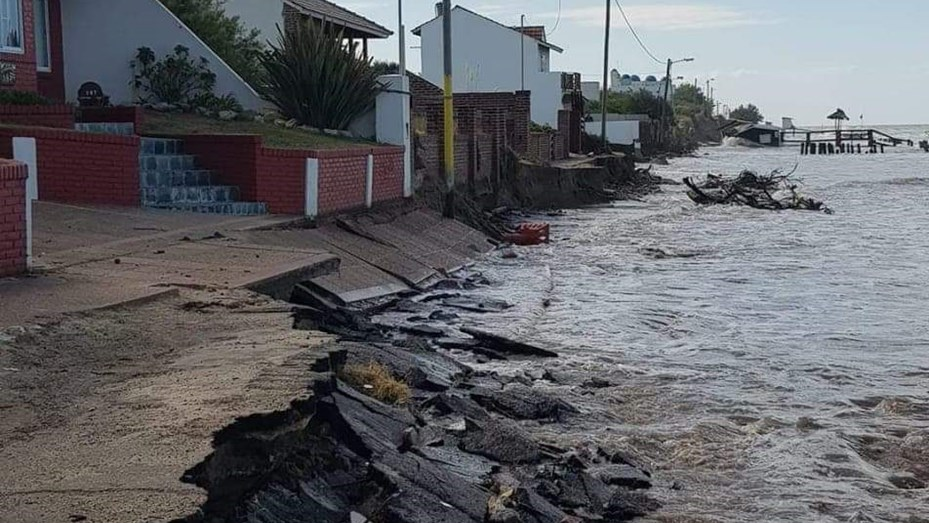
\includegraphics[width=3.64583in,height=\textheight]{./img/image49.jpeg}
\caption{Erosión costera en Las Toninas, Pcia. de Bs. As.}
\end{figure}

Podrían verse afectadas algunas de las planicies de marea en la costa al
sur de Bahía Blanca, como Bahía Anegada y Bahía San Blas y la zona sur
de la Bahía Samborombón de gran riqueza en su biodiversidad.

En la costa marítima, las playas acotadas por acantilados o por
asentamientos urbanos y forestación, podrían perder su extensión
gradualmente, e incluso desaparecer, afectando su valor turístico.

\begin{figure}
\begin{minipage}{0.48\textwidth}

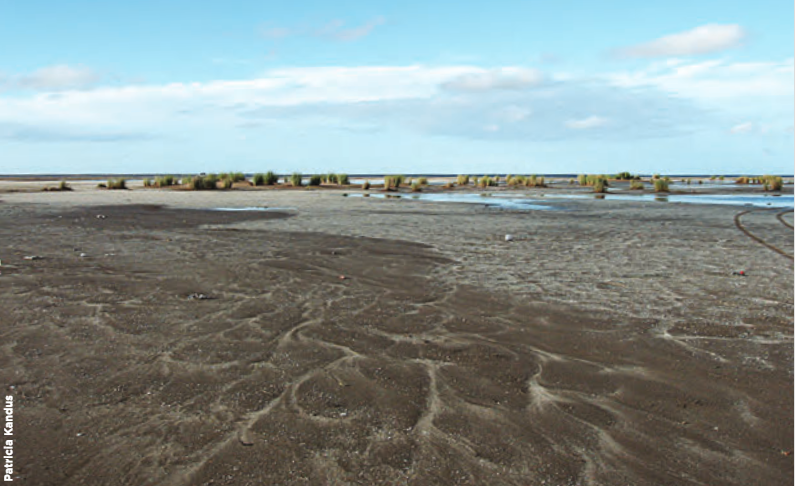
\includegraphics[width=3.64583in,height=\textheight]{./img/image50.png}

\caption{ Planicies de marea en la costa bonaerense. }
\end{minipage}\hfill%
\begin{minipage}{0.48\textwidth}

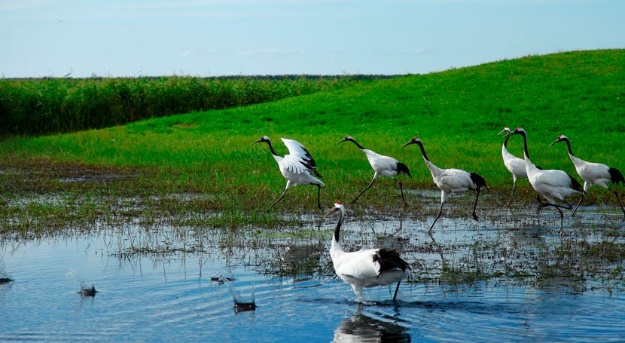
\includegraphics[width=3.64583in,height=\textheight]{./img/image51.jpeg}

\caption{ Zona de humedales}
\end{minipage}
\end{figure}

El aumento del nivel medio del mar tiene impacto directo sobre los
sistemas costeros debido a que son afectados por una mayor frecuencia de
inundaciones, procesos erosivos, pérdida de humedales, intrusión de agua
salada, etc.

Se espera que el calentamiento global continúe en el futuro (incluso más
allá del siglo 21) por lo que todos estos cambios continuarán, en
conjunto con una mayor recurrencia de fenómenos climáticos extremos.

\begin{figure}
\centering
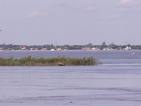
\includegraphics[width=2.08333in,height=\textheight]{./img/image53.jpeg}
\caption{El IPCC lanzó reportes para adelantarse al manejo de eventos
extremos del clima exacerbados por el cambio climático. Fuente:
\url{https://www.ipcc.ch/report/managing-the-risks-of-extreme-events-and-disasters-to-advance-climate-change-adaptation/}}
\end{figure}

Las regiones de arrecifes de corales han sido afectadas por un proceso
llamado blanqueo o decoloración.

El incremento en la temperatura de los océanos se considera la causa más
probable. Al estar más caliente el mar las algas, que viven de forma
simbiótica con el coral, abandonan al coral que las acoge. Las algas
proporcionan nutrientes y color para el coral. Sin ellas, el coral se
blanquea o decolora.

\begin{figure}
\centering
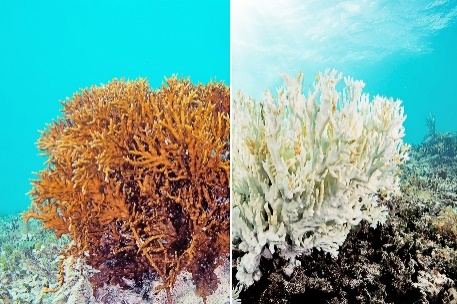
\includegraphics[width=4.16667in,height=\textheight]{./img/image55.jpeg}
\caption{Decoloración en los arrecifes.}
\end{figure}

\begin{figure}
\centering
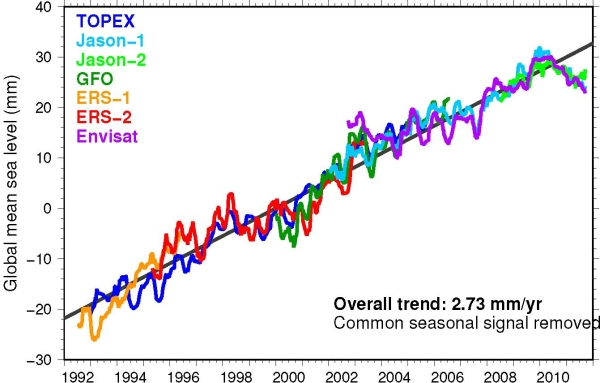
\includegraphics[width=4.16667in,height=\textheight]{./img/image56.jpeg}
\caption{Tendencias del Nivel del Mar (NM), medidas por sistemas
satelitales, Fuente: IPCC,2014}
\end{figure}

El IPCC para correr sus modelos numéricos necesita establecer distintos
escenarios futuros. Los escenarios son descripciones coherentes y
consistentes de cómo el sistema climático de la Tierra puede cambiar en
el futuro.

Existen escenarios que son derivados de las posibles emisiones futuras
de gases de efecto invernadero, los cuales se utilizan en modelos
numéricos para el cálculo de proyecciones climáticas. Cualquier
descripción posible del clima futuro dependerá de las hipótesis
planteadas sobre las emisiones futuras de los gases de invernadero y
otros agentes contaminantes.

Escenarios climáticos

RCP: Representation Concentration Pathways

La temperatura media aumentaría en todo el país durante este siglo,
tanto en un escenario de aumento de las concentraciones de GEI moderado
(RCP4.5) como de aumento extremo (RCP8.5).

\begin{figure}
\begin{center}
\begin{minipage}{0.6\textwidth}

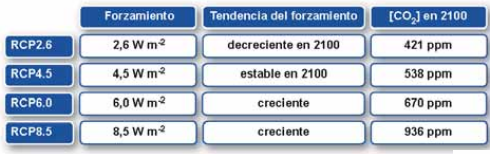
\includegraphics[width=4.16667in,height=\textheight]{./img/image57.png}

\caption{Escenarios climáticos posibles según IPCC}
\end{minipage}
\begin{minipage}{0.6\textwidth}

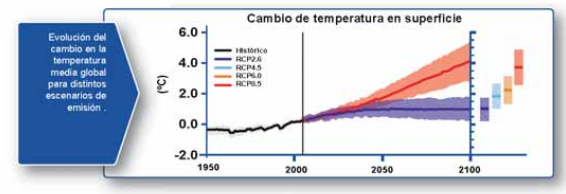
\includegraphics[width=4.16667in,height=\textheight]{./img/image58.png}

\caption{ Proyecciones de temperatura.}
\end{minipage}
\end{center}
\end{figure}

Basada en las proyecciones de temperatura realizadas por el IPCC para
diferentes escenarios. Todas las proyecciones son mayores que las
estimadas para el 2100 en el AR4.

Fuente: Rodriguez Camino (2009).

\hypertarget{cuxe1lculo-de-tendencias-del-nivel-del-mar-en-la-costa-argentina}{%
\subsubsection{Cálculo de tendencias del Nivel del Mar en la costa
Argentina}\label{cuxe1lculo-de-tendencias-del-nivel-del-mar-en-la-costa-argentina}}

\begin{figure}
\begin{center}
\null\hfill\begin{minipage}{0.7\textwidth}

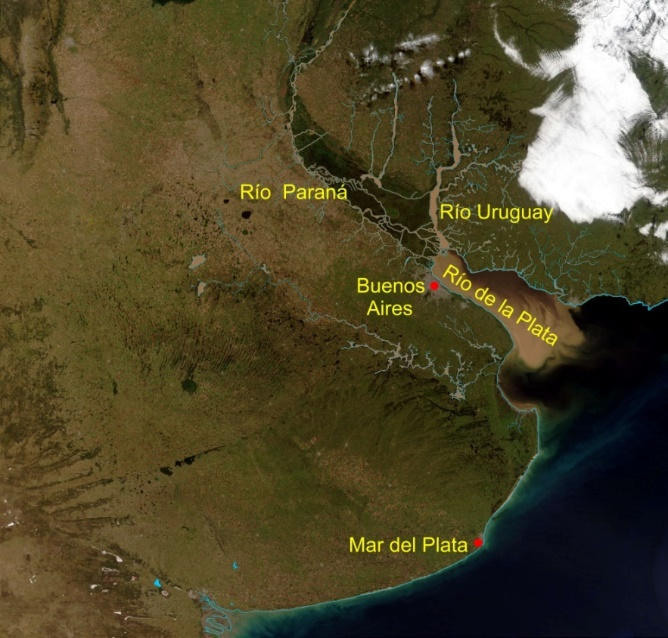
\includegraphics{./img/image59.jpeg}

\end{minipage}\hfill\null
\begin{minipage}{0.48\textwidth}

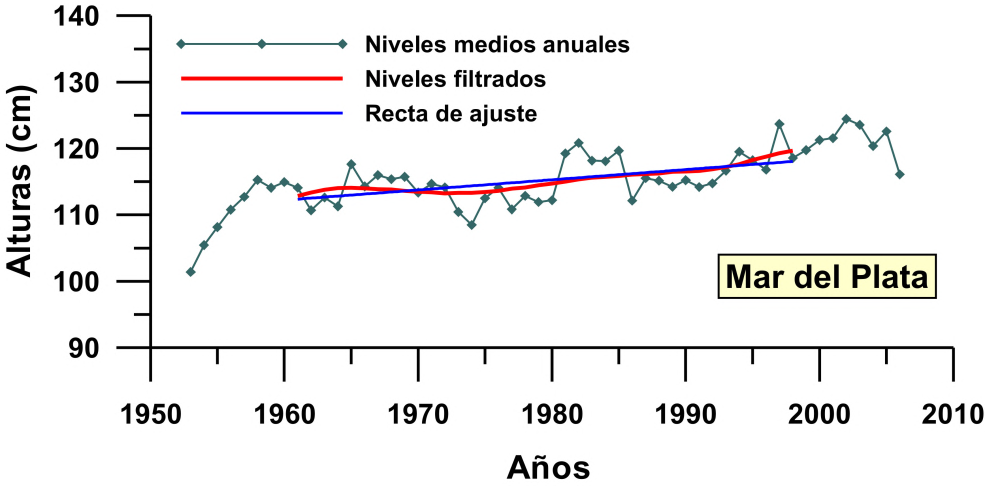
\includegraphics{./img/image60.png}

\caption{Tendencia en Buenos Aires 1,53 ± 0,11 mm/año}
\end{minipage}%\hfill
\begin{minipage}{0.48\textwidth}

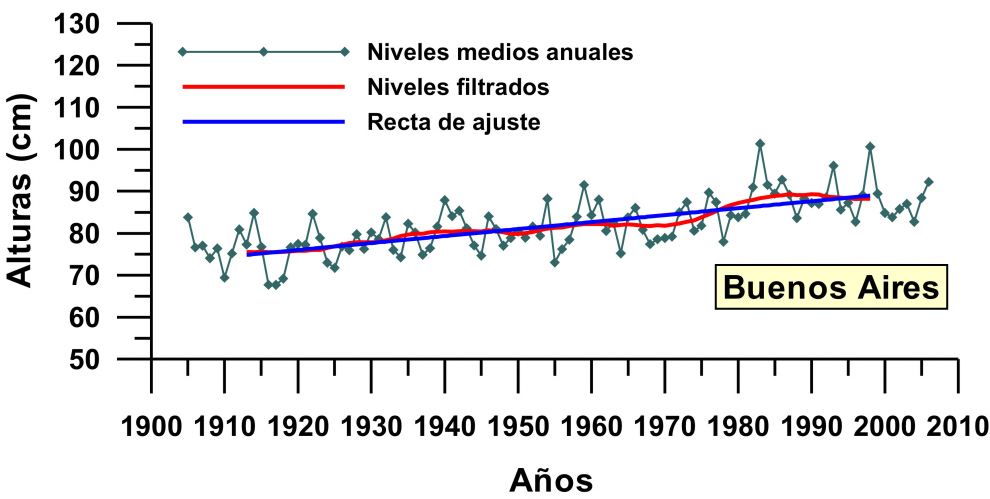
\includegraphics{./img/image61.png}

\caption{Tendencia en Buenos Aires 1,67 ± 0,05 mm/año}
\end{minipage}
\end{center}
\end{figure}

\begin{figure}
\centering
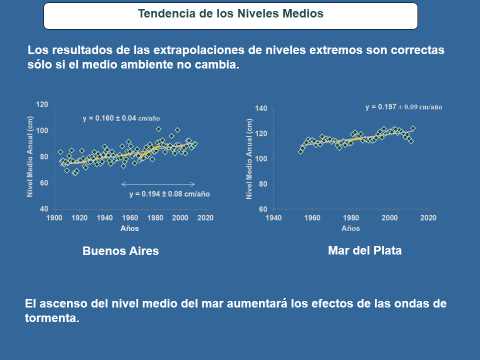
\includegraphics{./img/image62.png}
\caption{Otras Tendencias: Quequén: +1,6 ± 0,2 mm / año, Puerto Madryn:
+3,5 ± 0,1 mm / año}
\end{figure}

\begin{figure}
\centering
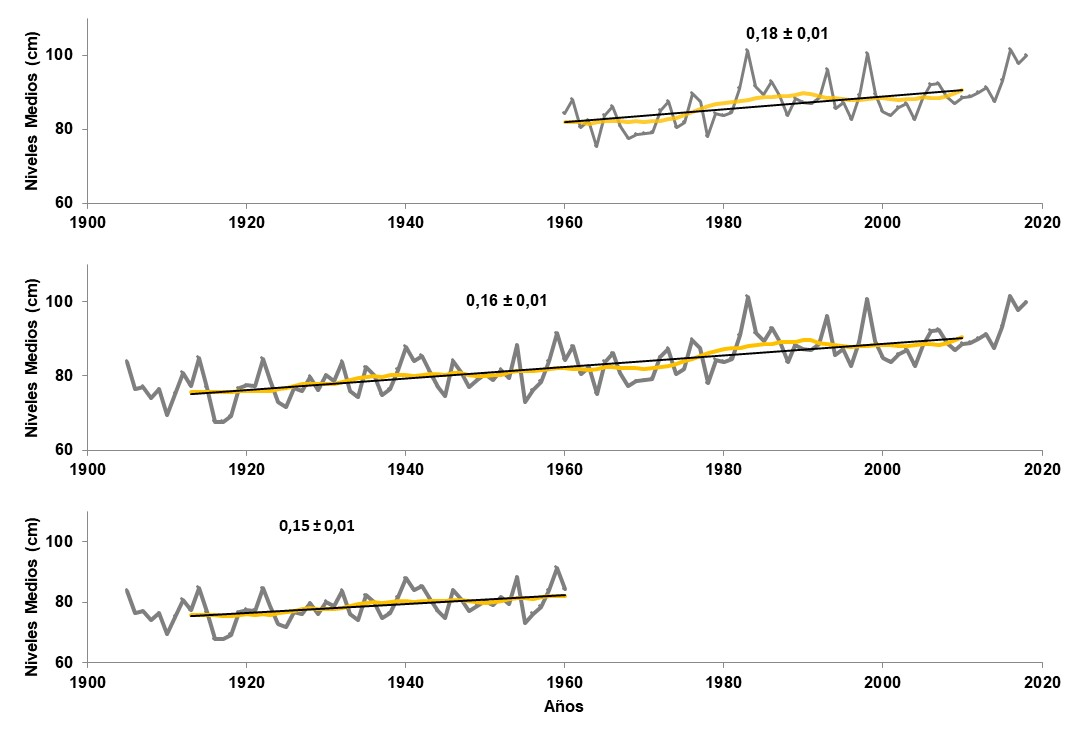
\includegraphics{./img/image63.jpeg}
\caption{Bs. As., Tendencia del nivel del Río de la Plata}
\end{figure}

\end{document}
